%        -----------------------------
%        | Group Assignment Template |
%        -----------------------------
%         Author: Zhong Tiantian
%         Date Created: Feb 21, 2022
%         Date Modified: Feb 22, 2022
%         Version: 2.0
%
% -------------------------------------------

\documentclass[12pt]{article}
\usepackage[scale=0.8]{geometry}
\usepackage{fontspec}   % 启用自定义字体
\usepackage{fancyhdr}
\usepackage{graphicx}   % 支持图像
\usepackage{hyperref}   % 支持引用(书签引用)
\usepackage{amsmath}    % 支持数学
\usepackage{amsfonts}   % 支持数学字体
\usepackage{amssymb}    % 支持数学符号
\usepackage{enumerate}
\usepackage{bm}
\usepackage{mathptmx}
\usepackage[nofillcomment, linesnumbered,ruled,lined,boxed]{algorithm2e}% 支持伪代码
\usepackage{listings}
\usepackage{fontspec}
\usepackage{booktabs}
\usepackage{tikz}
\usetikzlibrary {graphs, graphdrawing}
\usegdlibrary {trees}

% \everymath{\displaystyle}
\setmainfont{Times New Roman}
% \setmonofont{Consolas}
% \setsansfont{Arial}
\lstset{                  %设置代码块
    basicstyle=\small\fontspec{Consolas},% 基本风格
    numbers=left,    % 行号
    numbersep=10pt,  % 行号间隔
    tabsize=4,       % 缩进
    extendedchars=true, % 扩展符号?
    breaklines=true, % 自动换行
    frame=shadowbox,  % 框架左边竖线
    xleftmargin=19pt,% 竖线左边间距
    showspaces=false,% 空格字符加下划线
    showstringspaces=false,% 字符串中的空格加下划线
    showtabs=false,  % 字符串中的tab加下划线
}
\pagestyle{fancy}
\fancyhf{}
\fancyhead[L]{\textsc\COURSECODE \\ \textbf\HWTITLE}
\fancyhead[C]{}
\fancyhead[R]{Last Modified on \\ \today}
\fancyfoot[L]{\AUTHOR}
\fancyfoot[C]{}
\fancyfoot[R]{--\thepage--}

\fancypagestyle{firstPage}{
    \fancyhf{}
    \fancyfoot[R]{--\thepage--}
}

\newcommand{\E}{\text{e}}
\newcommand{\Diff}{\text{d}}

\title{\textsc\COURSECODE \\ \textbf{\HWTITLE}}
\author{\AUTHOR}
\date{\textit{\normalsize Last Modified on \today}}

\newenvironment{questions}{\begin{enumerate}[Ex. 1]}{\end{enumerate}}
\newenvironment{parts}{\begin{enumerate}[(i)]}{\end{enumerate}}
\newcommand{\question}[1]{\newpage \item \textsc{\textbf{Our Answer.}} (This part is written by #1)\newline}
\renewcommand\part{\item}
\newcommand\makeMyTitle{\maketitle
                        % Please add the following required packages to your document preamble:
% \usepackage{booktabs}
\begin{table}[htp]
    \centering
    \begin{tabular}{@{}clc@{}}
        \toprule
        \multicolumn{2}{c}{\textbf{Members}}                                                               \\ \midrule\midrule
        \multicolumn{1}{c|}{\textbf{Name}}  & \textbf{Student ID} \\ \midrule
        \multicolumn{1}{c|}{Li Rong}        & 3200110523          \\
        \multicolumn{1}{c|}{Zhong Tiantian} & 3200110643          \\
        \multicolumn{1}{c|}{Zhou Ruidi}     & 3200111303          \\
        \multicolumn{1}{c|}{Jiang Wenhan}   & 3200111016          \\ \bottomrule
    \end{tabular}
\end{table} 
                        \vspace{5cm}
                        \centering\textsc{\Large{Please turn over for our answers.}}\normalsize}

\renewcommand{\baselinestretch}{1.2}
% \setlength{\parskip}{0ex}



\def\HWTITLE{Homework 3}
\def\COURSECODE{CS 225: Data Structures}
\def\AUTHOR{Group D1}


\begin{document}
\makeMyTitle
\thispagestyle{firstPage}

\begin{questions}
    \question
    \begin{parts}
        \part
        Firstly we set the doubly linked list whose node's values follows the correct sequence. For operation \texttt{delete\_min} or \texttt{delete\_max}, we simply delete the first or last node of the linked lists. Then we set the value of  previous node pointer of the second element to\texttt{NULL} or  the value of  next node pointer of the last but second element to \texttt{NULL}. For insert operation, for example in a max heap, we traverse from the value of the first node until we reach a node whose value is smaller than the insert one. Then we set its previous node's next pointer to the inserted node and set the current node's previous node pointer to the inserted node. Finally we set the next node pointer of the inserted node to the current node and the previous node pointer of the inserted node to the last traversed node. For \texttt{decrease($h$,$k$)} operation, we traverse the doubly linked list and check its key value until we find the $h$'s node and decrease its value by $k$. Then we traverse the following nodes (for the sequence from big to small) to find the correct position for the node $h$, then we insert it to the correct position and delete the primal node.

        \part
        For insert and decrease operation, the time complexity for unsorted list is $O(1)$ .For sorted list, the time complexity is $O(n)$ . For delete operation, time complexity for both unsorted lists and sorted lists are $O(1)$ .


    \end{parts}

    \question
    \begin{parts}
        \part
        Each time we could compare the new element with the element in the lowest level. If the new element is smaller than the element in the heap, we could put this new element at the bottom of the heap. If the new element is bigger than the element in the heap, we should exchange the elements: put the new element in the original position of the element in the heap and move the original element in the heap to the bottom. Then we should compare the new element with the parent leaf in that position. Repeat this step until it mets a element in the heap which is bigger than the element or the new element is the biggest, we should put it at the top of the heap. For each new element we could repeat this process until we have finished inserting all the elements.

        \part
        \textbf{NOTE: We suspect that the given complexity is incorrect.}

        \paragraph{Original} There are $n$ elements in \texttt{maxHeap} and $k$ new elements to insert.

        

        \paragraph{Step 1:} Take the example shown in Figure \ref{fig-inserting}. We put the new elements at the bottom of \texttt{maxHeap}.

        \paragraph{Step 2:} We calculate the parent node which has two children (the yellow node). There are $[k/2]$ elements initially, and then there are $[k/4]$ elements because of those $[k/2]$ elements, and then $[k/8]$ elements... , $ \sum_{i=1} k/2^i=k $, For them, we can use the thought of the heap, we should spend $O(k)$ time to build heap.

        \paragraph{Step 3:} We now calculate the father node with only one child node(the blue node). It's like a link with the property of the heap though it doesn't have other nodes to amortize the sift-down node. So there are at most $\log(n)$ nodes, with each node $\log(n+k)$ time to form a heap (So far, we cannot consider them as a heap as it is like a link without other branch nodes, as a result we can neither consider the time complexity as $O(\log(n))$. So the total time complexity is $\log(n)\log(n+k)\approx O(\log(n)\log(n+k))$.

        Therefore, the final time complexity is $O(k+\log(n)\log(n+k))$ rather than $O(k+\log(n))$.

        % \paragraph{Inserting New Nodes.} We append the new nodes to the binary heap, maintaining its properties as a complete binary tree. This indicates that there are at most one nodes whose number of children is 1.

        % \begin{tikzpicture}
        %     \caption{Inserting $k$ elements to the bottom of a heap.}
        %     \centering
        %     \tikz [tree layout, sibling distance=8mm, mark/.style={fill=violet, text=white}, mark/.default=, markmin/.style={fill=red, text=white}, markmin/.default=]
        %     \graph [nodes={circle, draw, inner sep=1.5pt}]{ [fresh nodes]

        %     a

        % \end{tikzpicture}


    \end{parts}

    \begin{figure}[h]
        \centering
        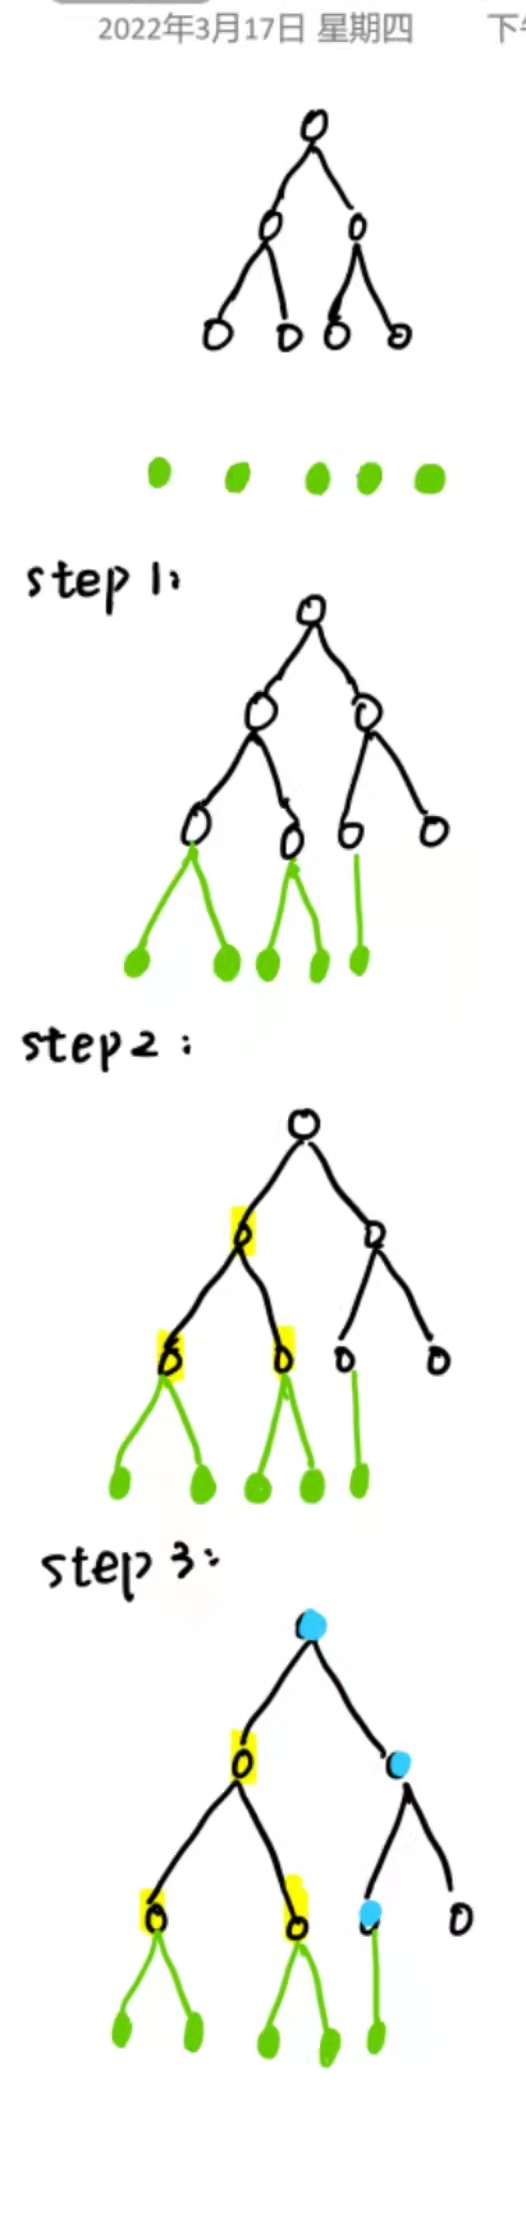
\includegraphics[width=4cm]{fig_inserting.jpg}
        \caption{The example inserting process for Ex. 2.}

        \label{fig-inserting}
    \end{figure}

    \question
    \begin{parts}
        \part
        The \texttt{siftUp} operation requires $\log(n)$ comparisons, each layer requires one. At each layer, compare the leaf node with parent node and swap the leaf node and parent node if needed. Therefore the time complexity is $O(\log_{n})$ . For insert operation, we add the inserted node to the end of the heap. Then we apply \texttt{siftUp} operation to it until the property of heap is gained.

        \part
        Firstly we find the larger leaf node for each layer and it takes $\log{n}$ times of comparison. Then we set up a list consists of these values and the amount is $\log{n}$ , then we apply binary search to find the proper position. It takes $O(\log{\log{n}})$ steps to accomplish. Thus, the steps needed is $\log{n}+O(\log{ \log {n}})$ .
    \end{parts}
\end{questions}

\end{document}